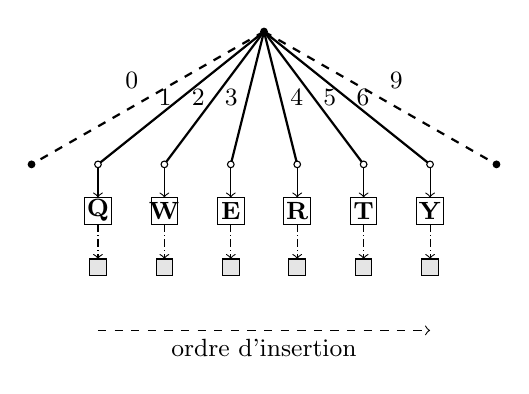
\begin{tikzpicture}[scale=1.2]

  %% node to node
  \small
  \draw[dashed, thick] (0pt,0pt) -- node[anchor=south east]{0} (-70pt,-40pt);
  \draw[thick] (0pt,0pt) -- node[anchor=east]{\DARKBLUE{1}} (-50pt,-40pt);
  \draw[thick] (0pt,0pt) -- node[anchor=east]{\DARKBLUE{2}} (-30pt,-40pt);
  \draw[thick] (0pt,0pt) -- node[anchor=east]{\DARKBLUE{3}} (-10pt,-40pt);
  \draw[thick] (0pt,0pt) -- node[anchor=west]{\DARKBLUE{4}} ( 10pt,-40pt);
  \draw[thick] (0pt,0pt) -- node[anchor=west]{\DARKBLUE{5}} ( 30pt,-40pt);
  \draw[thick] (0pt,0pt) -- node[anchor=west]{\DARKBLUE{6}} ( 50pt,-40pt);
  \draw[dashed, thick] (0pt,0pt) -- node[anchor=south west]{9} ( 70pt,-40pt);

  %% node to element
  \draw[->] (-50pt,-40pt) -- (-50pt,-50pt);
  \draw[->] (-30pt,-40pt) -- (-30pt,-50pt);
  \draw[->] (-10pt,-40pt) -- (-10pt,-50pt);
  \draw[->] ( 10pt,-40pt) -- ( 10pt,-50pt);
  \draw[->] ( 30pt,-40pt) -- ( 30pt,-50pt);
  \draw[->] ( 50pt,-40pt) -- ( 50pt,-50pt);

  %% element to desambiguator
  \draw[->,densely dashdotted] ( -50pt,-58pt) -- ( -50pt,-68.5pt);
  \draw[->,densely dashdotted] ( -30pt,-58pt) -- ( -30pt,-68.5pt);
  \draw[->,densely dashdotted] ( -10pt,-58pt) -- ( -10pt,-68.5pt);
  \draw[->,densely dashdotted] (  10pt,-58pt) -- (  10pt,-68.5pt);
  \draw[->,densely dashdotted] (  30pt,-58pt) -- (  30pt,-68.5pt);
  \draw[->,densely dashdotted] (  50pt,-58pt) -- (  50pt,-68.5pt);

  \draw[fill=black] (  0pt,  0pt) circle (1pt);
  \draw[fill=black] (-70pt,-40pt) circle (1pt);
  \draw[fill=white] (-50pt,-40pt) circle (1pt);
  \draw[fill=white] (-30pt,-40pt) circle (1pt);
  \draw[fill=white] (-10pt,-40pt) circle (1pt);
  \draw[fill=white] ( 10pt,-40pt) circle (1pt);
  \draw[fill=white] ( 30pt,-40pt) circle (1pt);
  \draw[fill=white] ( 50pt,-40pt) circle (1pt);
  \draw[fill=black] ( 70pt,-40pt) circle (1pt);

  %% elements
  \draw[fill=white](-50pt,-54pt)
  node{\textbf{Q}}+(-4pt,-4pt)rectangle+(4pt,4pt) ;
  \draw[fill=white](50pt,-54pt)
  node{\textbf{Y}} +(-4pt,-4pt) rectangle +(4pt,4pt) ;
  \draw[fill=white]( 10pt,-54pt)
  node{\textbf{R}} +(-4pt,-4pt) rectangle +(4pt,4pt) ;
  \draw[fill=white] ( -30pt,-54pt)
  node{\textbf{W}} +(-4pt,-4pt) rectangle +(4pt,4pt) ;
  \draw[fill=white] ( -10pt,-54pt)
  node{\textbf{E}} +(-4pt,-4pt) rectangle +(4pt,4pt) ;
  \draw[fill=white]( 30pt,-54pt)
  node{\textbf{T}} +(-4pt,-4pt) rectangle +(4pt,4pt) ;

  %% desambiguator
  \draw[fill=gray!20] (-50pt,-71pt) +(-2.5pt,-2.5pt) rectangle +(2.5pt,2.5pt);
  \draw[fill=gray!20] (-30pt,-71pt) +(-2.5pt,-2.5pt) rectangle +(2.5pt,2.5pt);
  \draw[fill=gray!20] (-10pt,-71pt) +(-2.5pt,-2.5pt) rectangle +(2.5pt,2.5pt);
  \draw[fill=gray!20] ( 10pt,-71pt) +(-2.5pt,-2.5pt) rectangle +(2.5pt,2.5pt);
  \draw[fill=gray!20] ( 30pt,-71pt) +(-2.5pt,-2.5pt) rectangle +(2.5pt,2.5pt);
  \draw[fill=gray!20] ( 50pt,-71pt) +(-2.5pt,-2.5pt) rectangle +(2.5pt,2.5pt);

  %% insertion order
  \draw[->,dashed] (-50pt, -90pt) -- node[anchor=north]{ordre d'insertion}
  (50pt, -90pt);

\end{tikzpicture}
